\section{Use Case Description}
  \subsection{General view}
The user should call the ray tracer engine providing a scene xml file. The parser will create the world objects. And finally the engine will render the image using the world objects.

\begin{figure}[ht]
  \centering
  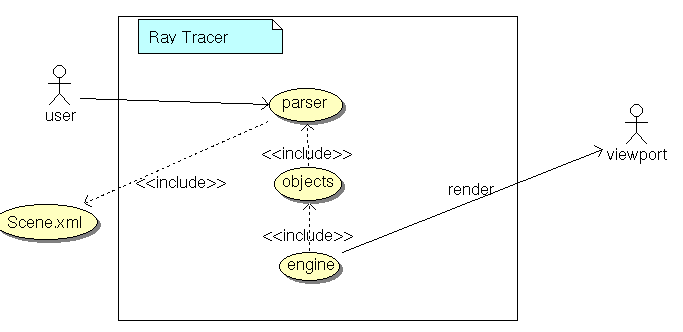
\includegraphics[height=9cm]{img/uc_raytracer.png}
  \caption{Use case general view}
  \label{img_uc_rt}
\end{figure}

  \clearpage
  \subsection{Objects}

The parser create all objects of the scene.

The creation of the camera also create the viewport.

\begin{figure}[ht]
  \centering
  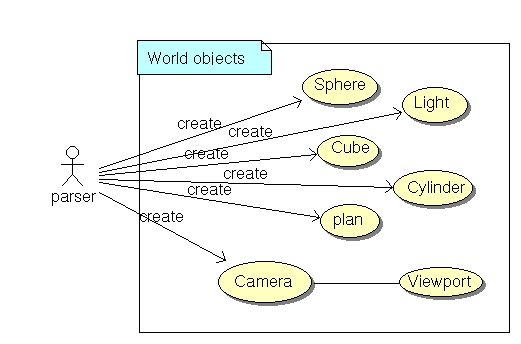
\includegraphics[height=9cm]{img/uc_objects.png}
  \caption{Use case objects creation}
  \label{img_uc_obj}
\end{figure}

  \clearpage
  \subsection{Engine}

Engine algorithm : for each pixel of the viewport, throw a ray and calculate the color where the ray intersect with an object.

\begin{figure}[ht]
  \centering
  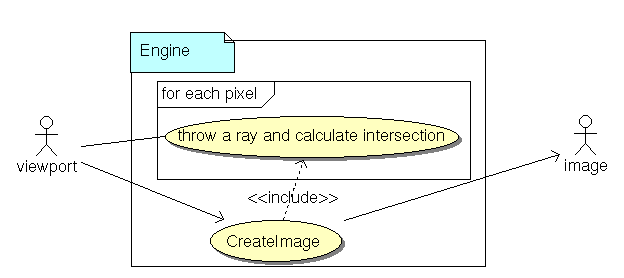
\includegraphics[height=7cm]{img/uc_render.png}
  \caption{Use case engine}
  \label{img_uc_engine}
\end{figure}


